\section{Implementation details and checks}
\label{sec:appendix}

\paragraph{Reproduction.}
\texttt{experiments/dirty\_paper/run.py -{}-self-test} checks four properties: the closest-vector search is never worse than brute force over a box in four dimensions; every A-null exact write leaves old outputs unchanged to \(10^{-8}\) and decodes all new items; as \(M\to\infty\) the precoded target equals GPM's; and the A-null precoder is never costlier than THP or than the coset reached by modular descent.
\texttt{run.py} writes \texttt{results.json} with every seed's norms, accuracy curves and decay curves; \texttt{papers/dirty-paper/plot.py} regenerates both figures, both tables and every number in the text from that file.

\paragraph{Interference and conditioning.}
The root-mean-square interference \(s_B\) is 4.1--4.6 at \(S=0\) and 21.5--29.4 at \(S=4\); the median condition number of \(G\) is 28--63.
Modular descent decoded every new item at its exact write in every seed.
The A-null closest-vector search was exact in every instance; the joint search was exact in at least \cvpexact{} of instances per configuration, and a capped search only overstates the joint arm's cost.

\paragraph{An uninformative probe.}
The first sweep also wrote four further tasks without protection after the \(B\) write.
Every arm, including GPM, fell to chance on both \(A\) and \(B\), so the probe could not separate them and was replaced by the weight-shrink curves in \cref{fig:decay}.

\begin{figure}[h]
  \centering
  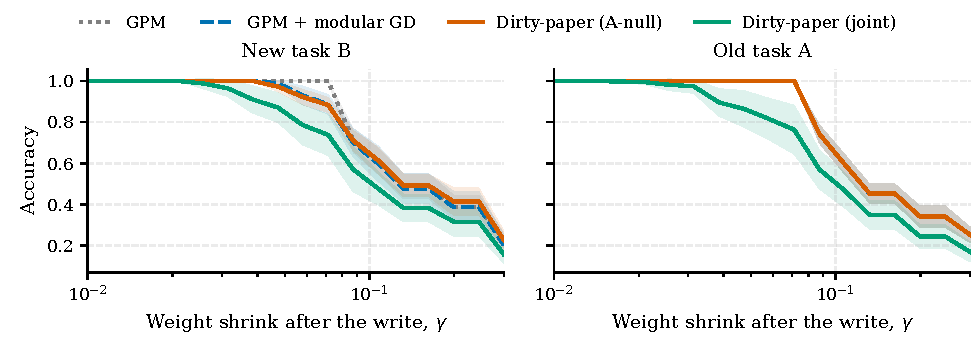
\includegraphics[width=\textwidth]{decay.pdf}
  \caption{\textbf{The joint write's old outputs are the first to fail under later training.}
  Accuracy after an exact write followed by a uniform weight shrink \(w\mapsto(1-\gamma)w\), at the main configuration.
  The A-null arms coincide on the old task; the joint arm, which moved old outputs by whole periods, loses them at smaller \(\gamma\).
  Means over \nseeds{} seeds with 95\% Student-\(t\) bands.}
  \label{fig:decay}
\end{figure}
